\documentclass[letterpaper,12pt,twoside]{report}% Use this line for the print version of the thesis
%\documentclass[12pt,oneside]{report}% If you comment out the line above, and uncomment this line, it will create a file without the extra pages that the Library wants for its electronic file versions.

\usepackage{byustyle}
\byustylesetup{%
  % Definitions of names needed in thesis/dissertation
  deptname          = School of Technology,
  committeechairman = Barry Lunt,
  committeemembera  = Derek L.\ Hansen,
  committeememberb  = Richard Helps,
  %graddate = April 2011,   % Final approval month (NOT graduation month!
   %
  %Uncomment to shorten for proofreading purposes
  %noabstract = true,         % Don't show the abstract page
  %nouniversitypages = true,  % Don't show any of the "university pages"
  %noacknowledgements = true, % Don't show the Acknowledgements page
  %notableofcontents = true,  % Don't show the Table of Contents
  %nolistoffigures = true,    % Don't show the List of Figures
  %nolistoftables = true,     % Don't show the List of Tables
  nonomenclature = true,      % Don't show the Nomenclature section - note that this section is optional
  %notocandlists = true,      % Don't show the Table of Contents, List of Figures, or the List of Tables
  keywords = {learning preference, cognition, LSI, computing, academic success, AMSS}
}

%%%%%%%%%%%%%%%%%%%%%%%%%%%%%%%%%%%%%%%%%%%%%%%%%%%%%%%%
%  Include other \usepackage{} statements here.
%    Add one package at a time.
%    Warning:  Some packages are not compatible with byuthesis.sty
%%%%%%%%%%%%%%%%%%%%%%%%%%%%%%%%%%%%%%%%%%%%%%%%%%%%%%%%%
% You should turn on any of these that you think you'll need!

%\usepackage[normalmargins]{savetrees}  % prints smaller to save trees (draft only)
\usepackage{amsmath}  % allows for mathematical symbols
\usepackage{amssymb}  % defines symbol names for all the math symbols
\usepackage{graphicx} % for .pdf graphics inclusion
\usepackage{caption}
\usepackage[calcwidth = \columnwidth]{caption}
\usepackage{booktabs,threeparttable}
\usepackage{subcaption}
\usepackage{setspace} % change the spacing inside a document
\usepackage{epstopdf} % converts a .eps to a .pdf
\usepackage{cite}     % allows for citations
\usepackage{mathptmx}
\usepackage{textcomp}
\usepackage{float}    % improves the interface for defining floating objects
\usepackage{rotating}

\usepackage[round]{natbib}
\usepackage{listings}
%\usepackage[figuresright]{rotfloat}
%\usepackage{multirow}
%These next two lines are for the citing with the IEEE style (leave commented for ASME)
%\renewcommand\citepunct{], [}
%\renewcommand\citedash{]--[}

\usepackage[pdftex,backref,pagebackref=false,plainpages=false]{hyperref}
\hypersetup{
  breaklinks  = false, % Allow link text to break across lines (default=false).
  linktocpage = false, % make page number, not text, be link on TOC, LOF and LOT
  colorlinks  = false, % Color the text of links (true) or put color frames over
  linkbordercolor = {1 1 1}, % The color of the box around normal links (white so they won't show up)
  citebordercolor = {1 1 1}, % The color of the box around citations (white so they won't show up)
  pdfstartview = {FitV}, % Set the startup page view. Possible options are:
                         % FitH: Fit whole width of page
                         % FitV: Fit whole height of page
                         % FitB: Fit whole Bounding Box page
                         % FitBH: Fit whole width of Bounding Box of page
                         % FitBV: Fit whole height of Bounding Box of page
  bookmarksnumbered  = true, % Put section numbers in bookmarks (default=false)
  bookmarksopen      = true, % Open up the bookmark trees (default=false).
  bookmarksopenlevel = 0, % Level to which bookmarks are open (default=\maxdimen).
  bookmarkstype      = toc, % Specify which toc file to mimic (default=toc).
  pdfpagemode        = {UseOutlines}, %  Specify how document starts when opened ({None}).
                                      % Possible options are:,
                                      % None: Neither bookmarks nor thumbnails are visible.
                                      % UseOutlines: Bookmarks are visible.
                                      % UseThumbs: Thumbnails are visible.
                                      % FullScreen: Full-screen mode
  pdftitle    = {Thesis},
  pdftitle    = {A Cognitive Approach to Predicting Academic Success in Computing},
  pdfauthor   = {Colby Goettel},
  pdfcreator  = {Colby Goettel},
  pdfsubject  = {Colby Goettel's Master's Thesis},
  pdfkeywords = {Master's Thesis, BYU, computing, academic success, LSI},
  pdfborder = {0 0 0},
}

%%%%%%%%%%%%%%%%%%%%%%%%%%%%%%%%%%%%%%%%%%%%%%%%%%%%%%%%
%  Define macros here - You may use these, or delete them, as you see fit.
%%%%%%%%%%%%%%%%%%%%%%%%%%%%%%%%%%%%%%%%%%%%%%%%%%%%%%%%%
\setcounter{tocdepth}{1}

% To remove bold fonts in TOC. However, as this currently is, the vertical spacing gets thrown off.
% \usepackage{titletoc}
% \titlecontents{chapter}
% [0pt]                               % left margin
% {}%
% {\contentsmargin{0pt}               % numbered entry format
%     \thecontentslabel\enspace%
%     }
% {\contentsmargin{0pt}}              % unnumbered entry format
% {\titlerule*[.5pc]{.}\contentspage} % filler-page format (e.g dots)
% []                                  % below code (e.g vertical space)

\DeclareCaptionJustification{InvertedPyramid}{\hsize=\linewidth
  \parindent=0pt
  \leftskip=0pt plus.5fil
  \rightskip=0pt plus-0.5fil
  \parfillskip=0pt plus1fil
  \emergencystretch=1in
  \parshape10
  0.00in \linewidth
  0.025\linewidth 0.95\linewidth
  0.05\linewidth 0.9\linewidth
  0.075\linewidth 0.85\linewidth
  0.1\linewidth 0.8\linewidth
  0.125\linewidth 0.75\linewidth
  0.15\linewidth 0.70\linewidth
  0.175\linewidth 0.65\linewidth
  0.2\linewidth 0.60\linewidth
  0.225\linewidth 0.55\linewidth
  \strut
}
\renewcommand{\TPTminimum}{3in}
\captionsetup[table]{justification=InvertedPyramid}

\newsavebox{\tempbox}
\newlength{\tempwidth}

% %%%%%%%%%%%%%%%%%%%%%%%%%%%%%%%%%%%%%%%%%%%%%%%%%%%%%%
% To only print a few chapters without changing the reference numbers,
% uncomment the chapters you want
% %%%%%%%%%%%%%%%%%%%%%%%%%%%%%%%%%%%%%%%%%%%%%%%%%%%%%%
%\includeonly{chapter1}
%\includeonly{chapter2}
%\includeonly{chapter3}
%\includeonly{chapter4}
%\includeonly{chapter5}
%\includeonly{chapter6}
%\includeonly{chapter7}
%\includeonly{appendixa}
%\includeonly{appendixb}
%\includeonly{appendixc}
%\includeonly{appendixd}

%%%%%%%%%%%%%%%%%%%%%%%%%%%%%%%%%%%%%%%%%%%%%%%%%%%%%%%%
% Start Document
%%%%%%%%%%%%%%%%%%%%%%%%%%%%%%%%%%%%%%%%%%%%%%%%%%%%%%%%
\begin{document}

% Define Title & Author
% For a title of more than one line, use the \\ to break up the lines so they appear in an inverse pyramid shape.
%Also, make sure you use title case (upper case for most of the first letters of words)
\title{A Cognitive Approach to Predicting\\Academic Success in Computing} %Ira A. Fulton College\\ of Engineering and Technology}
\author{Colby Goettel}

% For displaying the BYU Thesis header
%  This command assumes that there are documents called abstract.tex and
%  acknowledgements.tex that will be included in the header
\showBYUHeader

% Include chapters of the thesis here: (Note that you should open the files chapter1.tex and chapter2.tex to
% see some of the important notes about how to do your thesis!)
\chapter{Introduction}\label{chp:chapter1}
Incoming freshmen struggle deciding which field they should enter. In computing, there are many fields to choose from and this can cause confusion for new students, especially because the fields are so closely related. For example, many students don't know the difference between computer science (CS), information systems (IS), and information technology (IT). It would be so nice to have a simple way to determine which field would best suit the student. But how do these fields differ? And how do these differences help us determine the right fit for incoming computing students?

One potential way to look at the differences among the various computing fields is to look at the characteristics of the students in each of these fields~--- especially how they prefer to learn. CS, IS, and IT all focus on different areas of computing and each requires a different skill set. Is it possible to predict in which computing discipline an incoming freshman would succeed based on their learning style preferences? Previous research has shown a correlation between learning preference and academic success for engineering students (Lunt, 1996), but does this correlation also exist for computing students?

In the early 1970s, Dr.\ David Kolb developed a cognitive model to represent learning preferences. His model works on a two-axis system: concrete experience (CE) versus abstract conceptualization (AC), and reflective observation (RO) versus active experimentation (AE). This two-axis spectrum is meant to describe a student's learning preferences.

The \textit{x}-axis, AE$-$RO, differentiates between students who prefer to learn by doing, being active, seeing results, and those who prefer to learn by watching, listening, taking their time, and relying on observations. The \textit{y}-axis, AC$-$CE, differentiates between students who prefer to learn by thinking things out, reasoning, being rational, and those who are more intuitive and prefer to trust their feelings.

It doesn't appear that any research has been done in this area, \textit{viz}.: examining if a student's cognitive learning preference is a factor in which computing discipline they should study. Some of the research is close, but most deal with programming aptitude or success in a first year program. Interestingly, hardly any research has taken a cognitive approach. Finally, no research was found that focused on the differences between CS, IS, and IT.

\section{Purpose}
The purpose of this research is to discover if there is a correlation between a student's preference for AC$-$CE and AE$-$RO and their GPA, and overall satisfaction in CS, IS, and IT. This research matters because incoming freshman interested in computing struggle to decide between the various, computing majors. If there is a statistically significant correlation between Kolb's learning styles and success in CS, IS, and IT, then advisement centers could use the LSI to help incoming students choose among computing majors.

\section{Research questions}
\begin{itemize}
  \item How strong is the correlation between AC$-$CE and AE$-$RO, and major GPA among CS, IS, and IT students?
  \item How strong is the correlation between AC$-$CE and AE$-$RO, and student satisfaction among CS, IS, and IT students?
  \item Is there a correlation between major GPA and student satisfaction?
  \item What is the best multiple regression model to fit these correlations?
\end{itemize}

\section{The computing disciplines}
The Association for Computing Machinery (ACM) has defined five disciplines in computing~(Shackelford, 2006): computer engineering, computer science, information systems, information technology, and software engineering. Although there is overlap between disciplines, each discipline fills its own niche. Computer engineering is focused on designing and building computer hardware and its associated software. Computer science creates low-level software, and is also concerned with the theoretical principles of computing. Software engineering is primarily focused on creating highly reliable software systems. Information technology solves general computer problems and fulfills the organizational need to integrate systems. Information systems also fulfills an organizational need, but mostly from the management side.

\section{What is cognition?}
David Kolb created the Experiential Learning Theory (ELT)~(Kolb, 2005a) and used this theory as the basis for his Learning Style Inventory (LSI). This theory has its roots in famous cognitivists and learning philosophers like Dewey, Piaget, Jung, Freire, and Carl Rogers.

Kolb said that ``[l]earning is best conceived as a process, not in terms of outcomes''~(Kolb, 2005a). In this view, learning is more about the journey than the outcome. This is important because the ELT focuses on how ``[l]earning is the process of creating knowledge''~(Kolb, 2005a). This view is based on the Constructivist Theory of learning which says that a learner must construct new knowledge, or as Kolb said, ``[S]ocial knowledge is created and recreated in the personal knowledge of the learner''~(Kolb, 2005b). It's contrasted with the Transmission Model whereby ``pre-existing fixed ideas are transmitted to the learner''~(Kolb, 2005a).

This might seem like a purely semantic difference, but there's an important distinction between constructivism and transmission, much like there's an important distinction between learning as a process and learning as the end result. This is important because the ELT and this research focus on learning as a process: it matters \emph{how} students learn, not simply \emph{what} they learn.

\section{What is satisfaction?}
Satisfaction is how pleased a student is with their major decision. In order to be quantified, satisfaction was rated by the Academic Major Satisfaction Scale which was developed and validated in 2007 by Margaret Nuata. It contained questions that asked the student to rate how happy they were with their major, if they considered changing majors, and how they felt about their major:
\begin{enumerate}
  \item ``I often wish I hadn't gotten into this major.
  \item I wish I was happier with my choice of an academic major.
  \item I am strongly considering changing to another major.
  \item Overall, I am happy with the major I've chosen.
  \item I feel good about the major I've selected.
  \item I would like to talk to someone about changing my major''~(Nuata, 2007).
\end{enumerate}

\section{Delimitations}
This research was limited to seniors because they have been exposed to myriad professors and courses, giving them a well-rounded view of the institution. Furthermore, this research was limited to CS, IS, and IT students at BYU because there are too many confounding variables to properly deal with other schools and their admissions processes in a study of this size.

This research did not look at the socioeconomic backgrounds of the students involved. It did not consider any social pressure students may receive to join a particular field.

\chapter{Literature review}\label{chp:chapter2}
The literature review focused on studies already done on this topic, how previous studies in computing had incorporated cognitive theory, and what surveys should be used to assess a student's cognitive learning preference and their satisfaction with their major.

The literature review was performed through Google Scholar and Brigham Young University's Harold B.\ Lee Library website. The criterion for a study to be considered relevant was that it had to match at least one of the following criteria:
\begin{enumerate}
  \item The study had to be about predicting academic success of students. For initial research, the tools and measures were not important. Once the author had an idea of which tools to use, further research was done on the reliability and efficacy of the given tools, as well as research into any criticism of those tools.
  \item For studies involving cognitive learning preferences, the studies were limited to science, technology, engineering, or mathematics (STEM) majors. For studies on criticism of the research tools, the search was expanded to include other disciplines because of the lack of relevant studies among the computing disciplines.
  \item The study had to be on students, not organizations. Additionally, the study could not be on a specific demographic subgroup of students (e.g., only 21 year-old Asian students whose parents have PhDs). Some studies were performed in niche environments and those qualities are noted in the following reviews.
  \item There was no requirement for the study to examine previous experience, high school performance, or tools like the SAT or ACT.
\end{enumerate}

The initial literature review was to find studies related to cognitive learning preference and how it affected STEM students. Upon finding that there was bountiful research in the area, the literature review was focused on finding studies related to cognitive preference among STEM students. Then, the literature review was expanded to include studies on academic success. Finally, the literature review focused on tool validation.

\section{Learning theories}
\subsection{Top-down and bottom-up}
In 2003, Ron Sun published a paper entitled Top-down versus bottom-up learning in cognitive skill acquisition(Sun, 2004). This paper looked at two different cognitive learning styles. These styles, respectively, were about whether acquiring knowledge was from a general idea to a specific idea, or vice versa. As important as this idea is, Sun's paper had no independent research to back it up.

\subsection{Acquisition and participation metaphors}
Sfard mentioned two metaphors for learning~(Sfard, 1998): acquisition metaphor (AM) and participation metaphor (PM). AM says that people learn by learning (as opposed to doing). Facts, ideas, and concepts build on each other. These pieces of information~--- referred to as objects~--- are colloquially known as knowledge. Knowledge is then internalized and stored in memory. Historically, AM has been the metaphor used for thousands of years to describe knowledge and learning. Generally, when people think about learning, they are thinking about the AM.

PM is a learning style dictated by actions: people learn by doing. PM advocates teach that knowledge is not something that people have, it's societal and communal: learning is done by being part of a community. This type of learning is all-encompassing, meaning that learning isn't something that someone has, it's one part of the whole.

\subsection{Atkinson-Shiffrin model of memory}
\begin{figure}
  \centering
  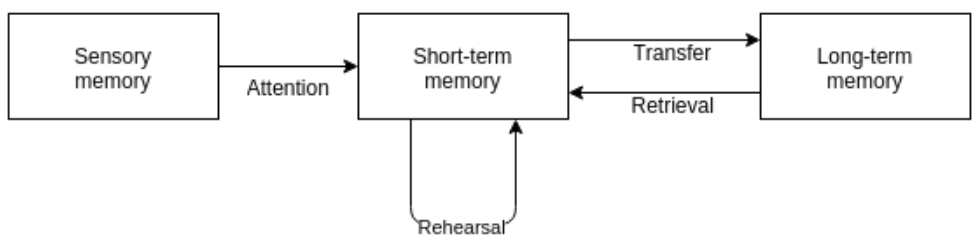
\includegraphics[width=\textwidth]{figures/chapter2/atkinson-model-of-memory.png}
  \caption{The Atkinson-Shiffrin Model of Memory}
  \label{fig:atkinson-model-of-memory}
\end{figure}

The Atkinson-Shiffrin model of memory is shown in Figure~\ref{fig:atkinson-model-of-memory}. The premise is that as individuals pay attention to sensory stimulation, short-term memories are created. As short-term memory is rehearsed and transferred, it turns into long-term memory. As long-term memory is retrieved, it comes into short-term memory so that it can be used.

The major components of this model are some form of input, storage, retrieval, and (eventually) forgetting. When presented with information, an individual must input and store the information. This creates short-term memory. If this memory is rehearsed (retrieved) often, it has a chance to become long-term memory. Neurologically speaking, when memories are rehearsed, the myelin sheaths of neurons form along certain pathways making memory. However, like muscle, if these memories are not used, they are lost.

This model works as a basic model of human learning because learning is the internalization of knowledge in long-term memory. If an individual has successfully internalized and retrieved knowledge, they have learned. In education, this is the predominant reason why exams exist: exams test students to see if they have learned the concepts taught in a class.

The Atkinson-Shiffrin model of memory shows the basic process by which people store information, but lacks the depth necessary to properly portray pedagogy. Learning is more than memorization: it's also internalization and application.

\subsection{Vygotsky's learning models}
According to Vygotsky~(Vygotsky, 1978), learning is not something people have, it's something they do. Learning is participatory. It is experiencing something that happened in the world. This is incredibly close to how David Kolb defined learning: ``[T]he process whereby knowledge is created through the transformation of experience''~(Kolb, 2013).

In contrast to learning, development is the actual progress being made by the learner. Development is the fruits of learning. In Vygotsky's mind, there are two types of development: actual development and proximal development. Actual development is what a learner can do. Proximal development, however, is the distance between what a learner can do on their own versus what they can do with someone more knowledgeable than themselves. This more knowledgeable person is not necessarily a master of their domain, but a peer or a teacher — they just have to be someone more knowledgeable in the learner's domain.

Vygotsky theorized that learning is experiences had in the world: learning happens all the time. In fact, everyone in the world that directly or indirectly influences the learner contributes to learning. This idea of communal learning, influenced by Marxism, is the idea that learners interact with others who already know how to live in the society; and learners learn how to live in their society through these interactions. Communal learning makes up a huge part of Vygotsky's idea of cultural apprenticeship, apprenticeship having more to do with interacting than coaching.

Because Vygotsky came from a communist nation, his thinking is heavily influenced by Marxist ideas. A prevalent, Marxist idea at his time was called Sovietization: if you can make someone live like a communist, they will think like a communist. This worked right into Vygotsky's collectivist thinking and influenced his ideas on social reproduction and enculturation: we become like the community when we learn to think and act like them. This cultural learning is not restricted to schooling because a lot of learning happens outside of school and especially before formal schooling begins. Children begin learning long before school: learning about their culture, their surroundings, their family.

Vygotsky thought of learning as a verb, not a noun: learning is not necessarily something that is had, it's something that is done. This works perfectly into the participation metaphor. He theorized that development is what a child is capable of doing: development is the fruit of learning. Vygotsky believed that what a child can do with others is more indicative of their development than what they can do alone.

Vygotsky was so radically different than his predecessors that he started an entire movement. The idea that learning is what influences development was in stark contrast to previous theorists who either believed that development came first or that learning and development were intertwined. Vygotsky changed the way people think about learning and was hugely influential in informing the learning theories used in this research.

\subsection{Experiential Learning Theory}
The Experiential Learning Theory (ELT), a cognitive approach to learning, was started by David A. Kolb in the 1970s and has continued to be updated with modern research since~(Kolb, 2005a). This theory and its related survey, the Kolb Learning Style Inventory (LSI), have been used and validated repeatedly since their creation. In fact, the survey is currently in its fourth major release.

Kolb says that ``[l]earning is best conceived as a process, not in terms of outcomes''~(Kolb, 2005a). In this view, learning is more about the journey than the outcome. This is important because the ELT focuses on how ``[l]earning is the process of creating knowledge''~(Kolb, 2005a). This view is based on the Constructivist Theory of learning which says that a learner must construct new knowledge, that is to say, ``[S]ocial knowledge is created and recreated in the personal knowledge of the learner''~(Kolb, 2005b). It's contrasted with the Transmission Model whereby ``pre-existing fixed ideas are transmitted to the learner''~(Kolb, 2005a).

This might seem like a purely semantic difference, but there's an important distinction between constructivism and transmission, much like there's an important distinction between learning as a process and learning as the end result. This is important because the ELT and this research focus on learning as a process: it matters how students learn, not simply what they learn. For these reasons, the ELT was chosen as the basis for assessing cognitive preference.

\section{Related studies}
\subsection{Lunt's \textit{Predicting Academic Success in Electronics}}
Lunt's dissertation, \textit{Predicting Academic Success in Electronics}~(Lunt, 1996), was foundational for this thesis. It performed the same research being performed here, but with an older version of the Kolb Learning Style Inventory (LSI), a focus on the electronics fields, and no focus on major satisfaction.

The purpose of Lunt's research was to determine if there was a correlation between learning style preference and academic success in electronics technology, electronics engineering technology, and electrical engineering. If there was a statistically significant correlation, then the LSI could be used as an accurate discriminator to help students choose in which electronics program they should enroll.

The students were randomly sampled and there was a participation rate of 45\%. Because the students were randomly sampled and the participation rate was $>$10\%, inferences to the population could be drawn.

The research questions were:
\begin{enumerate}
  \item ``What are the best predictor variables for predicting academic success in electronics?
  \item Is abstract learning preference an effective discriminator between students in the three main types of electronics programs?
  \item What is the best multiple-regression model that can be derived for predicting success in each of the three types of electronics programs?''~(Lunt, 1996)
\end{enumerate}

This rationale was persuasive because it focused on the differences between various majors in the same field and it was aimed at helping students determine which major to choose. Additionally, the Kolb LSI is a tested and validated tool for determining cognitive preference. Finally, the Experiential Learning Theory (ELT) on which the test is based fits right in line with the ideas behind this research.

The multiple regression model presented found correlations which helped justify the need to expand this line of research to computing students.

The paper's claims were justified in light of the methods used and it drew many interesting implications. This paper found that AC-CE~--- a Kolb axis measured by the LSI~--- is a good discriminator and can be used to help potential electronics students choose a major.

\subsection{Other studies}
There were several non-cognitive studies~(Thomas, 2007; Elnagar, 2013; Ridgell, 2004; Ting, 2001) that were foundational in understanding the scope of research done in this field. Other studies focused on previous academic success~(Barlow-Jones, 2011; Golding, 2005; Ting, 2001; Campbell, 1984), programming or mathematics aptitude~(Nowaczyk, 1984; Evans, 1989), or other unrelated and non-cognitive models~(Barlow-Jones, 2011; Elnagar, 2013).

The most common non-cognitive tool used was the Non-Cognitive Questionnaire (NCQ); however Thomas found that ``none of the scales of the NCQ are adequate predictors of GPA or persistence in college''~(Thomas, 2007). Other non-cognitive tools included personality tests (e.g., Myers-Briggs Personality Type Indicator, 16 Personality Test), general knowledge tests (e.g., SAT, ACT), and work drive. In 2004, Ridgell studied these variables with great success ($p<0.01$) finding that the personality traits exam was found to statistically correlate with course grades and GPA. However, none of the tools Ridgell used were cognitively-based.

In the same vein, \textit{Predicting Academic Performance in the School of Computing \& Information Technology (SCIT)}~(Golding, 2005) looked at students' performance in first-year courses. This was useful because it looked at all courses a first-year student takes, not just programming courses as most studies did. The study also looked at demographic information and a student's qualification for entry to the school and aptitude test scores, neither of which are administered in the US. It then used these indicators, as well as a student's overall performance in the program, to predict their future performance. However, the study did not look at college entrance exam scores or high school GPA. This research found that none of the entrance exams used~--- including the SAT~--- were good predictors for academic success. It also found that high school success in math, science, and previous IS and IT classes were not good indicators for academic success. Mostly, this paper found that the then-current indicators for admission were incorrect and not statistically significant. The only positively-correlated finding was that first-year programming and networking classes were good indicators for later success~(Golding, 2005).

Historically, studies tried to determine academic success by a student's programming or math aptitude using surveys like the Fennema-Sherman Mathematics Attitude Scale~(Nowaczyk, 1984), the IBM Programmer Aptitude Test~(Hostetler, 1983), or even COBOL~(Nowaczyk, 1984) or FORTRAN~(Campbell, 1984) proficiency. However, these surveys were found to not be the most effective tools to determine future academic success with ``R-squares of less than 24 percent''~(Evans, 1989).

\section{Why cognition?}
The various studies already mentioned each take a non-cognitive approach to predicting academic success. Since previous studies have failed to look at cognition, it leaves a clear opportunity that this research can fill. Cognition might not be the right theory, but that needs to be addressed. Additionally, cognitive theory seems to be the best candidate because it focuses on how students think and interpret information which is key in understanding technical concepts.

\section{Cognitive learning preference}
In 2005, the Hay Group published \textit{Learning Styles and Learning Spaces: Enhancing Experiential Learning in Higher Education} which gave interpretations about the various learning styles in the LSI. This paper was useful because it is the foundation of some hypotheses, namely that CS and IS will be in different quadrants of the LSI. IT was not listed, although it falls roughly, but not squarely, into engineering. Since CS and management are in different quadrants, and IS is the management side of technology, it would follow that IS should probably be in a different quadrant. However, no information has been found supporting this claim so it's an important claim to test.

\section{Criticism of the LSI}
In 1990, DeCoux surveyed cognitive research on nursing students that used the LSI. This was done in an effort to determine if the LSI was a trusted assessment tool. DeCoux's research showed ``a lack of significant relationships between learning style and other variables,'' adding further that ``studies undertaken specifically to investigate the measurement properties of the LSI reported major criticisms which seem to have been ignored.'' Throughout the survey, DeCoux found that the LSI was ``the most frequently used method of measuring learning styles'' even though there were ``numerous charges of serious instrument weakness,'' concluding that ``[c]ontinued use of the Kolb LSI... as an experiential technique is not recommended''~(DeCoux, 2016).

More recent research has shown that ``[d]ifferent personality traits... and academic motivation... were found to be independently associated with student learning strategies''~(Donche, 2013). This study, covering more than 1,100 undergraduate students, found that teaching strategy was hugely impactful because of ``the importance of students' personality and academic motivation'' which were found to ``partly explain'' how students learn.

Despite these criticisms, the LSI has been widely used in previous research in this area and is still generally considered to be a valid learning style assessment tool. Most of the studies looked at as part of this literature review did not have negative things to say about the LSI, although they were not looking into the tool's validity. For these reasons, we have decided to adopt the LSI as the learning style assessment tool.

\section{Criticism of cognition and learning styles}
Wang and others looked into the correlation between Biggs' constructive alignment and how it affected students' learning approaches. This research went off the basis that ``university students' learning approaches... are highly correlated with students' achievement of learning outcomes''~(Wang, 2013). However, it then noted that ``[s]uch a statement... was underpinned neither by qualitative nor quantitative empirical data.'' Their research showed that a more constructively-aligned teaching environment ``would lead students to adjust their learning approaches'' so they could learn more deeply ``despite their pre-existing individual differences in the preferred learning approaches.'' Their research is important because it showed that learning preference, while not insignificant, could be forgone in order to learn deeply.

One of the main motivations fueling this research was the author's experience in IT and CS classes and how they so greatly differed. Because of the attitudes of the students in each major toward their courses and how the courses were taught, the author hypothesized that the cause of this schism was the learning styles of the students, so the author wished to pursue research in that realm.

\section{Defining satisfaction}
To assess student major satisfaction, Nuata's Academic Major Satisfaction Scale (AMSS) was used. Nuata created and validated this 6-item assessment in 2007 for her dissertation because there didn't seem to be an existing survey, noting that ``[s]urprisingly, studies investigating major satisfaction are fairly infrequent in the career-development literature''~(Nuata, 2007).

Over the course of her research, Nuata went through multiple iterations before landing on the six questions in the AMSS. After her first methodology which was comprised of 20 Likert-type questions, Nuata reformulated the AMSS into six Likert-type questions and found that ``[a]mong this new sample, Cronbach's alpha for the 6 AMSS items was .90. As in Study 1, this suggested that the items comprising the AMSS are fairly internally consistent''~(Nuata, 2007). Then in 2014, the AMSS was adapted for Korean students and re-validated~(Sovet, 2014). This helped show that the AMSS is a realistic and reliable tool for determining major satisfaction.

\section{Conclusion}
The literature was severely lacking in cognitive studies in computing. Every study found took a non-cognitive approach, looked at programming aptitude, or tried to use previous academic success and aptitude tests to predict future academic success. Furthermore, the literature almost exclusively focused on CS with IT and IS being either completely overlooked or an afterthought. This study helps fill the gap in research by providing a look into the cognitive learning preferences of computing students. Since there is no clear way to successfully predict academic success in computing, this research will help fill that gap by exploring a new avenue to predict academic success in computing.

\chapter{Methodology}\label{chp:chapter3}
\section{The Computing Disciplines}
The Association for Computing Machinery (ACM) has defined five disciplines in com\-put\-ing~(Shackelford, 2006): computer engineering, computer science (CS), information systems (IS), information technology (IT), and software engineering (SE). Although there is overlap between disciplines, each discipline fills its own niche. Computer engineering is focused on designing and building hardware and its associated software. Computer science creates low-level software, but is also concerned with the theoretical principles of computing. Software engineering is primarily focused on creating reliable software. Information technology also creates software, but mostly fulfills the organizational need to integrate systems. Information systems also fulfills an organizational need, but mostly from the management side.

Of the five computing disciplines, computer engineering is the least closely related to IT. SE is small in size nationwide and BYU doesn't even have an SE program. For these reasons, this study focused on CS, IS, and IT.

\section{Administration of Tests}
To distribute the surveys, the author gained permission from professors to enter the classrooms of predominantly senior-filled classes in CS, IS, and IT. Once in the classroom, he read the announcement script and distributed packets to each student. The packets contained a consent form, the demographic survey, the Kolb LSI, and the AMSS. It was necessary to distribute the surveys in class because the LSI is copyrighted.

\subsection{Consent Form}
The consent form was approved by BYU's Institutional Review Board (IRB). It contained information about the research and a place for students to sign granting access to their college transcripts. Additionally, the consent form contained information about the risks and benefits of the research, confidentiality, and what to do if a research subject had questions about the research.

\subsection{Kolb Learning Style Inventory}
The two most recent revisions of the Kolb Learning Style Inventory (LSI), versions 3.1 and 4, differ mainly in their analysis. As Kolb stated, ``[r]ecent theoretical and empirical work is showing that the original four learning styles—assimilating, converging, accommodating, and diverging—can be expanded to show nine distinct styles''~(Kolb, 2005b). Since this research was interested in how students differ in the ``original four learning styles,'' version 3.1 was used because it better focused on those differences.

The LSI is a twelve-question survey that takes between five and ten minutes to complete. The purpose of this tool is to determine the research subject's cognitive preference. The LSI charts cognition on a two-axis scale: concrete experience (CE) versus abstract conceptualization (AC), and reflective observation (RO) versus active experimentation (AE). In order to do this, the questions focus on if a person prefers to think, feel, observe, or experiment when learning, or any combination of those attributes. These terms are defined more completely in chapter four.

\subsection{Academic Major Satisfaction Scale}
Nuata's Academic Major Satisfaction Scale (AMSS) was used to assess the students' satisfaction. It contained six questions rated on a 5-point Likert-type scale with 1 being ``strongly disagree'' and 5 being ``strongly agree.'' The questions dealt with how the students felt about their choice of major, if they thought about switching majors, and if they would have liked to talk with someone about switching majors.

\subsection{Demographic Information}
The demographic survey asked about the students' gender, age, ethnicity, marital status, and parents' highest education.

\section{Participation Rate}
In \textit{The adequacy of response rates to online and paper surveys: what can be done?}, Nulty discussed the differences between online and paper surveys, including their response rates and how to improve them, and how to improve evaluation~(Nulty, 2008). The most important part of this study for this research was a table listing the needed participation rates for various class sizes. However, the paper stated that the table is ``only a guide as it is based on the application of a formula derived from a theory that has random sampling as a basic requirement''~(Nulty, 2008).

From Nulty's research, it was found that a participation rate of 35-48\% was necessary for a 10\% sampling error and 80\% confidence level. The CS and IS senior classes were estimated by their respective departments to be 100 students each, so participation from 21 students was necessary for each major. The IT senior class was estimated at 40 students, requiring participation from 16 students.

\section{Scoring Responses}
\subsection{Major GPA}
After the surveys were received, the author keyed each of the surveys, numbering the consent form and the LSI. The consent form was then torn off the packet and brought to the Registrar's Office. The registrar then took copies of each of the consent forms for their records. The registrar then looked up the student's major and major GPA, and e-mailed the unique number, major, and major GPA to the author in order to preserve anonymity from third parties.

\subsection{Kolb LSI (v3.1)}
The LSI presents twelve, multiple-choice style questions. For instance, the question might start out: ``When I learn, I prefer to:'' and then gives four options, one from each quadrant (i.e., AC, AE, CE, RO). Students then mark the options one through four according to their personal preference. These scores were then added together according to a specific algorithm to determine where each student fell on the two axes. These responses were then input into a spreadsheet and programmatically checked for data entry errors by ensuring that each row did not have repeat numbers and that all of the values entered equaled 120, as dictated by the algorithm. Once the totals for each axis were found, they were entered into the respective student's row on the main spreadsheet. Since the LSI does not use the individual scores to plot the student's learning preference on the AC$-$CE and AE$-$RO axes, additional columns were added to compute these differences.

These values are best explained by example. Student 6 in the study scored CE=24, RO=33, AC=23, and AE=40 so the computed values are AE$-$RO=7 and AC$-$CE=$-1$. This student is pretty squarely in the middle of the graph. They don't lean heavily towards any of the cognitive preferences, but instead prefer an equal mix of them all.

By comparison, I scored CE=48, RO=26, AC=21, and AE=25 so the computed values are AE$-$RO=$-1$ and AC$-$CE=$-27$. I'm moderate in the AE$-$RO axis~--- meaning I favor both active experimentation and reflective observation~--- but I'm strongly in the abstract conceptualization camp. This might seem counter-intuitive because I scored so high on CE, but I'm in the opposite (AC) end of the spectrum. This is because the individual scores aren't what matters: it's only the calculated values (i.e., AE$-$RO and AC$-$CE) that define cognitive preference.

\subsection{AMSS}
The AMSS is rated on a 5-point Likert-type scale with 1 being ``strongly disagree'' and 5 being ``strongly agree.'' This scale has both positively and negatively worded statements, the negatively worded statements being reverse scored. These scores were input into their own columns on the respective student's row.

\subsection{Demographic Information}
The demographic information was added as columns to each student's existing scores with consistent spelling and punctuation. Each answer was input in separate columns.

\chapter{Results}\label{chp:chapter4}
\section{Survey responses}
As discussed previously, a participation rate of 35-48\% was necessary for a 10\% sampling error and 80\% confidence level. This allowed for inferences to be made on the population, not just the students sampled. The CS and IS senior classes were estimated by their respective departments to be one hundred students each, so participation from twenty-one students was necessary for each major. The IT senior class was estimated at forty students, requiring participation from sixteen students. Table~\ref{tab:response-rates} shows the amount of responses received compared to the total amounts needed.

\begin{table}[h!]
  \centering
  \caption{Response Rates of Various Majors}
  \label{tab:response-rates}
  \begin{tabular}{llllll}
    \toprule
    Major & Total seniors in major & Surveys needed & Surveys received & Response rate\\
    \midrule
    CS    & 100                    & 35             & 40               & 40\%\\
    IS    & 100                    & 35             & 2                & 2\%\\
    IT    & 40                     & 14             & 22               & 55\%\\
    \bottomrule
  \end{tabular}
\end{table}

There were many complications getting responses from IS students. IS seniors do not have a capstone or senior seminar class, so there was no common opportunity to reach them. Since the Learning Style Inventory (LSI) is copyrighted and licensed for hardcopy use, it couldn't be digitized for distribution. This made it difficult to get surveys into the hands of the IS students. After trying for a year to get surveys out and being stonewalled by significant distribution problems, only two surveys from IS students were completed, and those were only completed because those students were in an IT course in which the surveys were distributed. No additional surveys were returned from IS students.

Because of the complications surrounding the IS responses, the IS results were not included in the analysis.

\section{What the LSI responses mean}
A student's strength on the two axes of the LSI can be seen in Figure~\ref{fig:learning-preferences} which defines the cognitive strengths throughout the LSI spectrum. These strengths can be either in abstract conceptualization (AC), active experimentation (AE), concrete experience (CE), reflective observation (RO), or along the AC$-$CE or AE$-$RO spectrums.

\begin{figure}
  \centering
  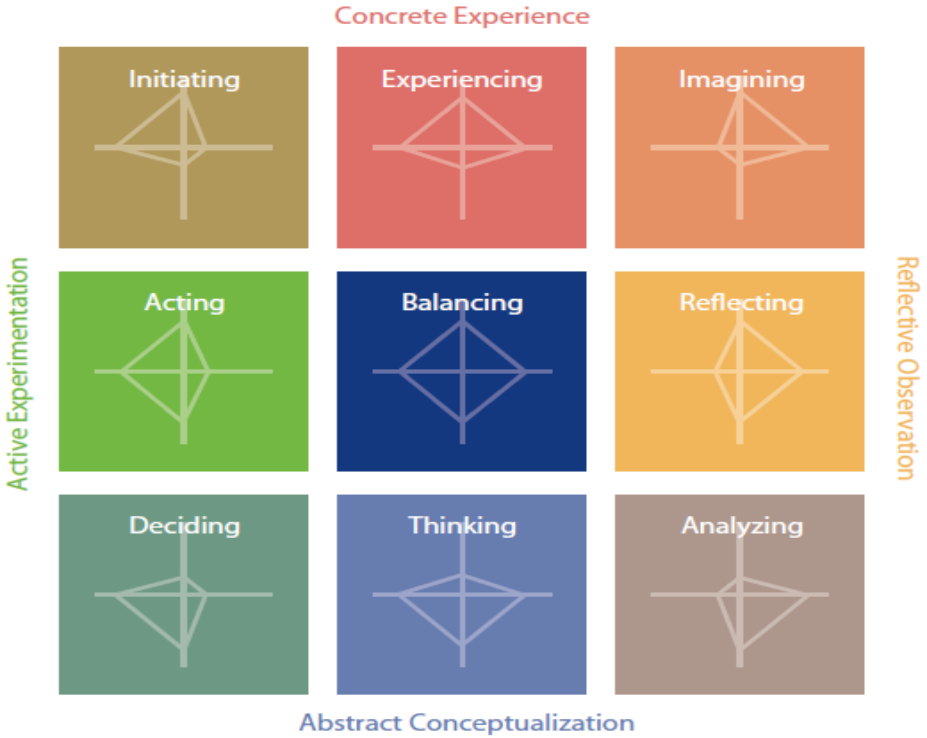
\includegraphics[width=0.9\textwidth]{figures/chapter4/learning-preferences.png}
  \caption{LSI Learning Preferences}
  \label{fig:learning-preferences}
\end{figure}

\subsection{Defining AC, CE, AE, and RO}
The terms abstract conceptualization, active experimentation, concrete experience, and reflective observation are not really intuitive. Before diving into the statistical analysis, it will be helpful to more clearly define these terms. The following list contains statements to help define each of these terms~(Kolb, 1993):
\begin{enumerate}
  \item Abstract conceptualization
  \begin{enumerate}
    \item To learn, I'd rather think about ideas.
    \item I'm logical.
    \item I like to reason things out.
    \item I want to analyze things.
    \item I'm rational.
    \item I rely on my ideas.
  \end{enumerate}
  \item Concrete experience
  \begin{enumerate}
    \item Thinking about my feelings affects how I learn.
    \item I trust my feelings and intuition.
    \item I'm open to experiencing new things.
    \item I like to learn from personal relationships.
    \item I like being actively involved in the learning process.
  \end{enumerate}
  \item Active experimentation
  \begin{enumerate}
    \item I want to be doing.
    \item I like to work hard.
    \item I want to see results.
    \item Just let me try it out myself.
    \item I'm practical.
  \end{enumerate}
  \item Reflective observation
  \begin{enumerate}
    \item I prefer to watch and listen.
    \item When I learn, I'm quiet.
    \item I take my time when I learn.
    \item I'm reserved.
    \item I like to look at issues from different angles.
    \item I'm observant.
    \item I prefer to slow down and be careful.
  \end{enumerate}
\end{enumerate}

\section{Examining the data}
Before answering the research questions, it's necessary to look at the data, get a feel for it, and visualize it. The first thing I did was run a $t$-test to see if there was a difference between CS and IT students' AC$-$CE and AE$-$RO scores. Each of these were statistically insignificant with $p>0.05$. This analysis is visualized in Figure~\ref{fig:cs-v-it-plot}. This is interesting because it goes against what the literature previously discussed about the relationship between learning styles, \textit{viz}.: CS and IT should be distinguishable~(Kolb, 2005b).

% TO LUNT: Would you like to see a table here, too? I think the figure is sufficient, but I'm willing to add a table of bad p-values if you think it would help.

\begin{figure}[!bhtb]
  \centering
  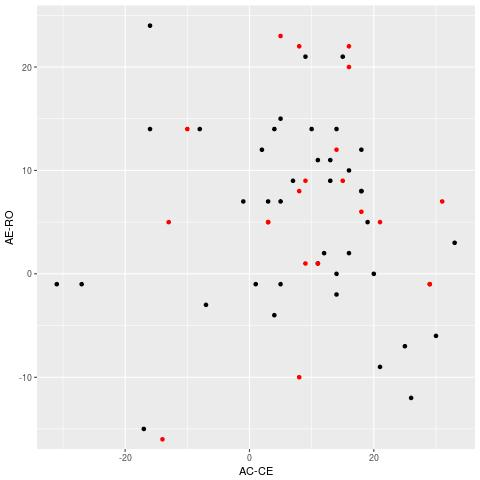
\includegraphics[width=0.7\textwidth]{figures/chapter4/cs-v-it-plot.jpg}
  \caption[AC$-$CE and AE$-$RO for CS and IT Students]{AC$-$CE and AE$-$RO for CS and IT Students Where Black is CS and Red is IT}
  \label{fig:cs-v-it-plot}
\end{figure}

Next, I needed to know if the data was normally distributed in order to determine which correlation model to run. To determine if the data was normally distributed, I ran the Shapiro-Wilk test, as noted in Table~\ref{tab:shapiro-wilk} (note that $p<0.05$ here means that the data is \emph{not} normally distributed). These findings will be discussed alongside the first research question.

\begin{table}[!htbp]
  \centering
  \caption{Shapiro-Wilk Tests}
  \label{tab:shapiro-wilk}
  \begin{tabular}{lll}
    \toprule
    Data         & W       & $p$-value \\
    \midrule
    CS major GPA & 0.95843 & 0.148 \\
    IT major GPA & 0.97703 & 0.8639 \\
    CS AC$-$CE     & 0.93586 & 0.0251 \\
    CS AE$-$RO     & 0.98255 & 0.7826 \\
    IT AC$-$CE     & 0.9529  & 0.3601 \\
    IT AE$-$RO     & 0.95844 & 0.4583 \\
    \bottomrule
  \end{tabular}
\end{table}

\section{Answering the research questions}
\subsection{How strong is the correlation between AC$-$CE and AE$-$RO, and major GPA among CS, IS, and IT students?}
Because all of these data points, except for CS AC$-$CE are normally distributed, I was justified in using Pearson's correlation coefficient (also known as Pearson's $r$) to calculate the correlations. This data is summarized in Table~\ref{tab:pearsons}.

\begin{table}[!htbp]
  \centering
  \caption{Pearson's $r$}
  \label{tab:pearsons}
  \begin{tabular}{lll}
    \toprule
    Data                      & $p$-value & $r$ \\
    \midrule
    CS major GPA and CS AC$-$CE & 0.8177    & -0.0376 \\
    CS major GPA and CS AE$-$RO & 0.6704    & -0.0694 \\
    IT major GPA and IT AC$-$CE & 0.9727    & -0.0077 \\
    IT major GPA and IT AE$-$RO & 0.0202    & 0.4915 \\
    \bottomrule
  \end{tabular}
\end{table}

Since CS students' AC$-$CE results were not normally distributed, I also ran Spearman's correlation coefficient to determine if there was a correlation between CS major GPA and CS AC$-$CE results. This resulted in $p>0.05$, but gave a warning that Spearman's shouldn't be used for data with tied values. To account for the tied values, I then ran the correlation using Kendall's $\tau_b$ which also had $p>0.05$.

Because of these findings, I am unable to find a statistically significant correlation between any major GPA and a student's LSI results, except for IT major GPA and IT AE$-$RO (see Figure~\ref{fig:major_gpa_lm_plots}). In fact, IT AE$-$RO is so strongly correlated to IT major GPA that it has an $R^2=r^2=0.4915^2=0.2416$. This means that an IT student's AE$-$RO score is able to explain 24.16\% of their GPA.

\begin{figure}
  \centering
  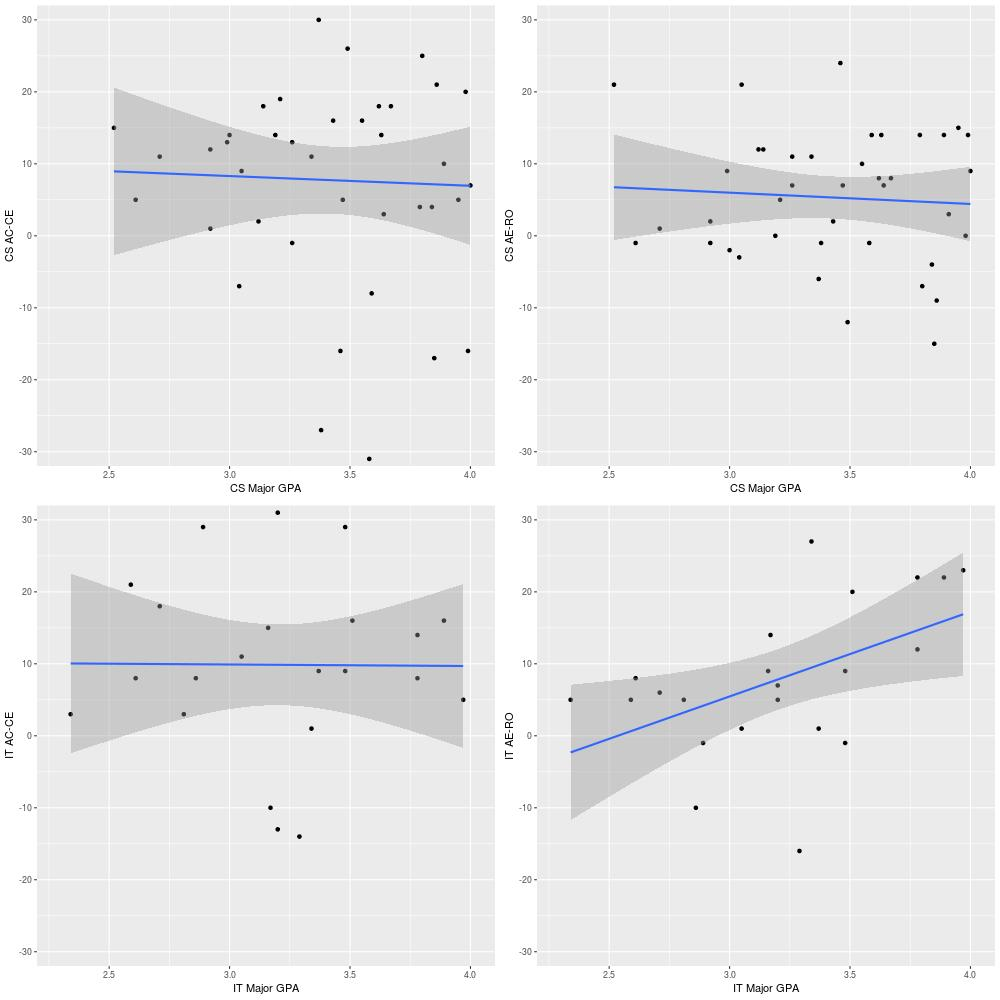
\includegraphics[width=1.1\textwidth]{figures/chapter4/major_gpa_lm_plots.jpg}
  \caption{Correlations Between Major GPA and LSI Results}
  \label{fig:major_gpa_lm_plots}
\end{figure}

The other important finding here is that there is a strong correlation between IT major GPA and IT AE$-$RO scores, such that the higher a student scores in the AE$-$RO spectrum, the higher we can assume their GPA to be. However, the AC$-$CE spectrum did not hold any statistically significant ($p>0.05$) effect on student GPA in CS or IT. This is interesting because Lunt found that AC$-$CE was the significant axis among electronics students~(Lunt, 1996).

% TO LUNT: I wrote this whole bit on looking at the IT major GPA data, but don't feel like it's necessary. I mean, it's a really pretty histogram, but it doesn't add to the overall argument. I wanted to make sure you were cool with me not including it before I just erased it.
% Looking at the IT major GPA data (in Table~\ref{tab:it-major-gpa}), it's clear that this data is normally distributed (note the Shapiro-Wilk $p=0.86$ from Table~\ref{tab:shapiro-wilk}; see Table~\ref{fig:it-major-gpa-hist}) with an almost equal mean ($\sigma=0.444$) and median. With this in mind, as well as the
%
% \begin{table}[!htbp]
%   \centering
%   \caption{IT Major GPA}
%   \label{tab:it-major-gpa}
%   \begin{tabular}{llllll}
%     \toprule
%     Min.  & 1st Qu. & Median & Mean  & 3rd Qu. & Max. \\
%     \midrule
%     2.340 & 2.868   & 3.200  & 3.204 & 3.480    & 3.970 \\
%     \bottomrule
%   \end{tabular}
% \end{table}
%
% \begin{figure}
%   \centering
%   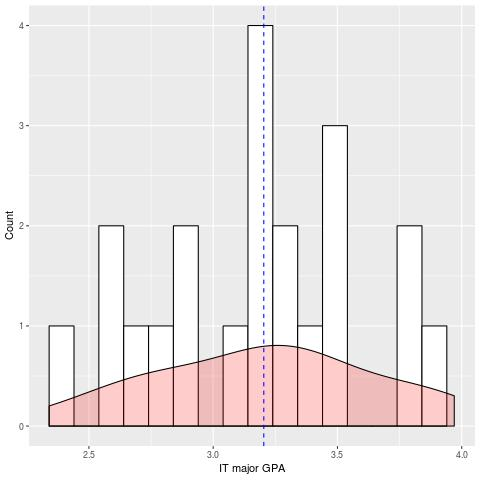
\includegraphics[width=0.7\textwidth]{figures/chapter4/it-major-gpa-hist.jpg}
%   \caption{IT Major GPA Histogram}
%   \label{fig:it-major-gpa-hist}
% \end{figure}

\subsection{What is the best multiple regression model to fit these correlations?}
In order to estimate the relationship that AC$-$CE and AE$-$RO each have simultaneously, I developed several multiple regression models. I ran these models with standard errors computed with the Huber-White (HC1) robust standard error to account for the heteroskedasticity of the data. The most significant models can be seen in Table~\ref{tab:mr-models}. All three models use major GPA as the dependent variable and compare that against the CS dummy variable (to determine is the student is a CS major), age, and parents education level. Model~2 adds AE$-$RO as a covariate, and Model~3 adds AC$-$CE as a covariate.

% Table created by stargazer v.5.2 by Marek Hlavac, Harvard University. E-mail: hlavac at fas.harvard.edu
% Date and time: Sun, Jan 28, 2018 - 01:49:51 PM
\begin{table}[!htbp] \centering
  \caption{Multiple Regression Models}
  \label{tab:mr-models}
  \begin{tabular}{@{\extracolsep{5pt}}lccc}
    \toprule
     & \multicolumn{3}{c}{\textit{Dependent variable:}} \\
    \cline{2-4}
    \\[-1.8ex] & \multicolumn{3}{c}{Major GPA} \\
    \\[-1.8ex] & (1) & (2) & (3)\\
    \midrule
    CS dummy variable & 0.110 & 0.137 & 0.137 \\
    &  &  &  \\
    Age 25-29 & $-$0.196 & $-$0.177 & $-$0.177 \\
    &  &  &  \\
    Age 30-34 & $-$0.443 & $-$0.425 & $-$0.426 \\
    &  &  &  \\
    Age 35+ & $-$0.096 & $-$0.077 & $-$0.082 \\
    &  &  &  \\
    Parents education --- & $-$0.661 & $-$0.667 & $-$0.667 \\
    \hspace{2em}some college &  &  &  \\[+0.5em]
    Parents education --- & $-$0.631 & $-$0.534 & $-$0.534 \\
    \hspace{2em}undergraduate degree &  &  &  \\[+0.5em]
    Parents education --- & $-$0.680 & $-$0.602 & $-$0.601 \\
    \hspace{2em}graduate degree &  &  &  \\[+0.5em]
    Parents education --- & $-$0.157 & $-$0.080 & $-$0.080 \\
    \hspace{2em}post-graduate degree &  &  &  \\[+0.5em]
    AE.RO &  & 0.007 & 0.007 \\
    &  &  &  \\
    AC.CE &  &  & 0.0002 \\
    &  &  &  \\
    Constant & 3.976$^{*}$ & 3.828$^{*}$ & 3.826$^{*}$ \\
    & (0.159) & (0.110) & (0.103) \\
    \midrule
    Observations & 62 & 62 & 62 \\
    $R^{2}$ & 0.367 & 0.389 & 0.389 \\
    Adjusted $R^{2}$ & 0.272 & 0.283 & 0.269 \\
    Residual Std. Error & 0.364 (df = 53) & 0.361 (df = 52) & 0.365 (df = 51) \\
    F Statistic & 3.848$^{*}$ (df = 8; 53) & 3.681$^{*}$ (df = 9; 52) & 3.250$^{*}$ (df = 10; 51) \\
    \bottomrule
    \textit{Note:}  & \multicolumn{3}{r}{$^{*}p<0.05$} \\
  \end{tabular}
\end{table}

These models each have statistically significant ($p<0.05$) F statistics, so I reject the null hypothesis that that these groups of variables do not have a statistically significant joint effect. However, an interesting thing happens between models~2 and~3: adding the AC$-$CE covariate decreases the adjusted $R^2$. This means that while the model is still significant with that covariate, it doesn't explain the variance as well. Again, this goes against what Lunt found concerning AC$-$CE results~(Lunt, 1996). The first two models can be seen in Figure~\ref{fig:mr_models_1_2}

\begin{figure}
  \centering
  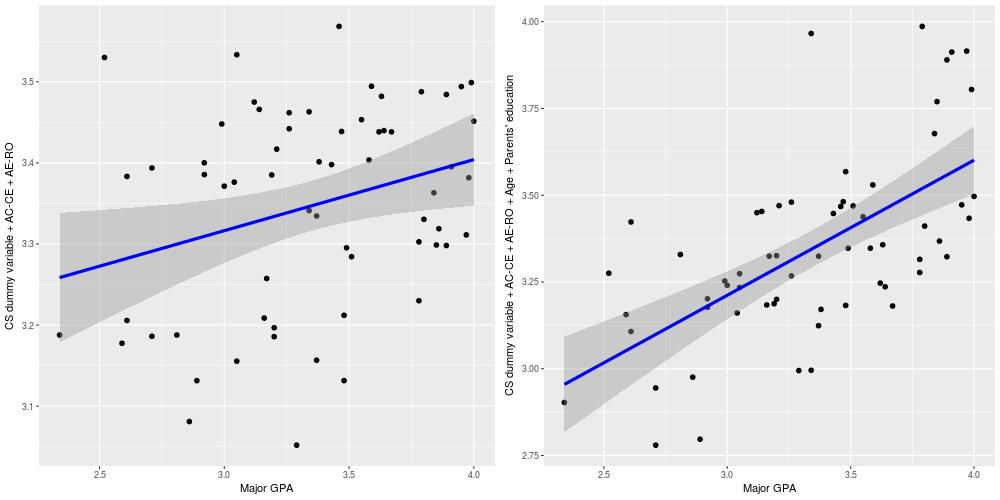
\includegraphics[width=1.1\textwidth]{figures/chapter4/mr_models_1_2.jpg}
  \caption{Multiple Regression Models 1 and 2}
  \label{fig:mr_models_1_2}
\end{figure}

Up to this point, I've only examined variables in groups, not individually. The linear hypothesis test compares the residual (error) sum of squares values against similar models. This way, I can check individual variables for a joint significance which will allow me to see if the variables can explain the deviance in the model. The null hypothesis is that each of these variables are 0. This test is important because removing unnecessary variables gives more power with this small of a dataset.

The model I ran used major GPA as the dependent variable, and compared it to the CS dummy variable, AE$-$RO, age, and parents education. This model had $p=1.266\times 10^{-10}$, so I reject the null hypothesis that these variables are not significant in explaining the variance in the data. This model reinforces the earlier, multiple regression findings.

\subsection{How strong is the correlation between AC$-$CE and AE$-$RO, and student satisfaction among CS, IS, and IT students?}
Nuata's AMSS, as enumerated in chapter 1, is graded on a five-point Likert-type scale with two of the responses being negatively scored. Two of the AMSS questions assume that students still have the option of changing their major, but once BYU students get beyond a certain credit threshold (well before their senior year), it becomes impossible for them to change majors. Because of this and the lack of variance among the responses, these questions were dropped from the analysis.

I created a summary index (Table~\ref{tab:nuata-summary-index}) of academic major satisfaction using the remaining AMSS variables and reverse coded the negatively-scored variables. In this summary index, the least satisfied value was a 4 and the most satisfied was a 20.

\begin{table}[!htb]
  \centering
  \caption{Summary Index of AMSS}
  \label{tab:nuata-summary-index}
  \begin{tabular}{cccccc}
    \toprule
    Min.  & 1st Qu. & Median & Mean  & 3rd Qu. &Max. \\
    \midrule
    12.00 &  16.25  & 19.00  & 18.10 & 20.00   & 20.00 \\
    \bottomrule
  \end{tabular}
\end{table}

Next, I checked the simple correlations between AE$-$RO and AC$-$CE with the satisfaction index. The Pearson coefficients are $-0.1206$ ($p=0.4645$) and $-0.0622$ ($p=0.7064$), respectively. It is possible that the relationship could only exist for the RO value, since this was the only value correlated with major GPA in the previous section. Checking for that, I found a Pearson correlation coefficient of $0.2634$ ($p=0.1051$). This means that even restricting to just RO and IT majors fails to find a statistically significant correlation ($0.2483$, $p=0.2652$).

None of these correlations were statistically significant, suggesting that there is no relationship between learning style and major satisfaction.

\subsection{Is there a correlation between major GPA and student satisfaction?}
The Pearson correlation coefficient of major GPA and the satisfaction index is $-0.1198$ ($p=0.4677$). This is statistically insignificant, so I am unable to say that there is a correlation between the two. The coefficient is negative, so if the correlation was significant it would indicate that students with higher major GPAs were generally less satisfied than students with lower GPAs.

% Add std dev
% Differentiate by major as well
The dataset, with four questions used, had a minimum sum of 4 (meaning the student strongly disagreed to each statement) and maximum sum of 20 (meaning the student strongly agreed with everything). The mean response was 18, so students were generally overwhelmingly satisfied with their choice of major. This lack of diversity is believed to have led to the lack of correlations between student satisfaction and other factors.

\section{Demographics}
Unfortunately, I was unable to use the full set of demographic variables collected from students as covariates because there was not enough variance among the sample group. The students were almost entirely white and male (88\% for both). Looking at the relationship between marital status and its relationship on major GPA and satisfaction had a multiple R-squared of $0.07$, and the relationship between marital status and RO and major GPA (previously the best model) had a multiple R-squared of $0.14$. So, while students were roughly equally divided in marital status, there was no relationship between marital status and any other factor.

\chapter{Conclusion}\label{chp:chapter5}
\section{Background}
Incoming freshmen struggle deciding which field of study they should enter. There are many computing fields and this can confuse new students who are interested in computing, especially because the fields are so closely related. For example, many students don't know the difference between computer science (CS), information systems (IS), and information technology (IT). It would be wonderful to have a simple way to determine which of these computing fields would best suit each student. How do these differences help us determine the right fit for incoming computing students?

One way to look at the differences among computing fields is to examine the students in each field~--- especially how they learn. CS, IS, and IT all focus on different areas of computing and each requires a different skill set. It seems like people in these fields have a preference for being taught differently. Is it possible to predict in which computing discipline an incoming freshman would succeed based on their learning style? Previous research has shown a correlation between learning preference and academic success, but does this correlation also exist for computing students?

In the 1970s, David Kolb developed a model to represent cognitive learning preference. His model works on a two-axis system: concrete experience (CE) versus abstract conceptualization (AC), and reflective observation (RO) versus active experimentation (AE). The \textit{x}-axis, AE-RO, differentiates between students who learn by doing or by seeing results, and those who prefer to learn by watching, listening, and taking their time. The \textit{y}-axis, AC-CE, differentiates between students who learn by reasoning and being rational, and those who prefer to trust their feelings.

The Association for Computing Machinery (ACM) has defined five disciplines in computing~(Shackelford, 2006): computer engineering, computer science (CS), information systems (IS), information technology (IT), and software engineering (SE). Although there is overlap between disciplines, each discipline is distinct. Computer engineering is focused on designing and building hardware. CS is concerned with the theoretical principles of computing, particularly the software. SE is focused on creating highly reliable software systems. IT solves general computer problems and focuses on systems integration. And IS fulfills an organizational need, but mostly from the management side.

\subsection{Research questions}
\begin{itemize}
  \item How strong is the correlation between AC-CE and AE-RO, and major GPA among CS, IS, and IT students?
  \item How strong is the correlation between AC-CE and AE-RO, and student satisfaction among CS, IS, and IT students?
  \item Is there a correlation between major GPA and student satisfaction?
  \item What is the best multiple regression model to fit these correlations?
\end{itemize}

\subsection{Defining terms}
Kolb created the Experiential Learning Theory (ELT)~(Kolb, 2005a) and used it as the basis for his Learning Style Inventory (LSI) assessment. According to this theory, learning is more about the journey than the outcome. This is important because the ELT focuses on how ``[l]earning is the process of creating knowledge''~(Kolb, 2005a). This view is based on the Constructivist Theory of learning: that a learner must construct new knowledge: ``social knowledge is created and recreated in the personal knowledge of the learner''~(Kolb, 2005b). It is contrasted with the Transmission Model whereby ``pre-existing fixed ideas are transmitted to the learner''~(Kolb, 2005a). This might seem like a purely semantic difference, but there's an important distinction between constructivism and transmission which is important because the ELT and this research focus on learning as a process: it matters how students learn, not simply what they learn.

Satisfaction is how pleased a student is with their decision on their major. In order to be quantified, satisfaction was rated by the Academic Major Satisfaction Scale, developed and validated by Nuata. It asks if students are happy with their major, if they think of switching majors, and how they feel about their choice.

\subsection{Delimitations}
Since IT is most closely related to CS and IS, and since BYU doesn't have an SE program, the study was limited to CS, IS, and IT.

\section{Literature review}
The purposes of the literature review were to determine if there were studies already done on this topic, how previous studies in computing had incorporated cognitive theory, and what surveys to use to study cognitive theory among computing students, including criticism of the chosen surveys.

The initial literature review was to find studies related to cognitive or learning preference and how it bears on STEM students. Upon finding that there was bountiful research in the area, the literature review focused on finding studies on cognitive preference. Then, research was expanded to include studies on academic success.

\subsection{Lunt's \textit{Predicting Academic Success in Electronics}}
Barry Lunt's dissertation, \textit{Predicting Academic Success in Electronics}, was foundational. It performed the same research being performed here, but with an older version of the LSI, a focus on the electronics fields, and no focus on major satisfaction.

The purpose of Lunt's research was to determine if there was a correlation between learning style preference and academic success in electronics technology, electronics engineering technology, and electrical engineering. If there was a statistically significant correlation, then the LSI could be used as an accurate discriminator to help students choose in which electronics program they should enroll.

The students were randomly sampled and there was a participation rate of 45\%. Lunt asked: ``What are the best predictor variables for predicting academic success in electronics? Is abstract learning preference an effective discriminator between students in the three main types of electronics programs? What is the best multiple-regression model that can be derived for predicting success in each of the three types of electronics programs?''~(Lunt, 1996)

This rationale was persuasive because it focused on the difference between various majors in the same field and it was aimed at helping students determine which major to choose. Additionally, the Kolb LSI is a tested and validated tool for determining cognitive preference. Finally, the Experiential Learning Theory (ELT) on which the test is based fits right in line with the ideas behind this present research.

The multiple regression model presented found correlations which helped justify the need to expand this line of research to computing students.

\subsection{Other studies}
There were several non-cognitive studies~(Thomas, 2007; Elnagar, 2013; Ridgell, 2004; Ting, 2001) that were foundational in understanding the scope of research done in this field. Other studies focused on previous academic success~(Barlow-Jones, 2011; Golding, 2005; Ting, 2001; Campbell, 1984), programming or mathematics aptitude~(Nowaczyk, 1984; Evans, 1989), or other unrelated and non-cognitive models~(Barlow-Jones, 2011; Elnagar, 2013).

The most common non-cognitive tool used is the Non-Cognitive Questionnaire (NCQ); however Thomas found that ``none of the scales of the NCQ are adequate predictors of GPA or persistence in college''~(Thomas, 2007). Other non-cognitive tools included personality tests (e.g., Myers-Briggs Personality Type Indicator, 16 Personality Test), general knowledge tests (e.g., SAT, ACT), and work drive. In 2004, Ridgell studied these variables with great success ($p<0.01$) finding that the personality traits exam was found to statistically correlate with course grades and GPA. However, none of the tools Ridgell used were cognitively-based.

In the same vein, \textit{Predicting Academic Performance in the School of Computing \& Information Technology (SCIT)}~(Golding, 2005) looked at students' performance in first-year courses. This was useful because it looked at all courses a first year student takes, not just programming courses (as most studies did). The study used demographic information and aptitude score, as well as a student's overall performance in the program, to predict their future performance. However, the study did not look at college entrance exam scores or high school GPA. This research found that none of the entrance exams used~--- including the SAT~--- were good predictors for academic success. It also found that high school success in math and science and previous IS and IT classes were not good indicators for academic success. Mostly, this paper found that the then-current indicators for admission were incorrect and not statistically significant.

Historically, studies tried to determine academic success by a student's programming or math aptitude, using surveys like the Fennema-Sherman Mathematics Attitude Scale~(Nowaczyk, 1984) and the IBM Programmer Aptitude Test~(Hostetler, 1983), or even COBOL~(Nowaczyk, 1984) or FORTRAN~(Campbell, 1984) proficiency. However, these surveys were found to not be the most effective tools to determine future academic success with ``R-squares of less than 24 percent''~(Evans, 1989) used in the study.

\subsection{Why cognition?}
These studies take a non-cognitive approach to predicting academic success. Since previous studies have failed to look at cognition, it leaves a gaping hole in the literature that needs to be filled. Cognition might not be the right theory, but that needs to be addressed. Additionally, cognitive theory is a good candidate because it focuses on how students think and interpret information, which is key in understanding technical concepts.

\subsection{Criticism of the LSI}
In 1990, DeCoux surveyed cognitive research on nursing students that used the LSI. This was done in an effort to determine if the LSI was a trusted assessment tool. DeCoux's research showed ``a lack of significant relationships between learning style and other variables,'' adding further that ``studies undertaken specifically to investigate the measurement properties of the LSI reported major criticisms which seem to have been ignored.'' Throughout the survey, DeCoux found that the LSI was ``the most frequently used method of measuring learning styles'' even though there were ``numerous charges of serious instrument weakness,'' concluding that ``[c]ontinued use of the Kolb LSI... as an experiential technique is not recommended''~(DeCoux, 2016).

More recent research has shown that ``[d]ifferent personality traits... and academic motivation... were found to be independently associated with student learning strategies''~(Donche, 2013). This study, covering more than 1,100 undergraduate students, found that teaching strategy was hugely impactful because of ``the importance of students' personality and academic motivation'' which were found to ``partly explain''~(Donche, 2013) how students learn.

Despite these criticisms, the LSI has been widely used in previous research in this area and is still generally considered to be a valid assessment tool. Most of the studies looked at as part of this literature review did not have negative things to say about the LSI, although they were not looking into the tool's validity. For these reasons, we have decided to adopt the LSI as the learning style assessment tool.

\subsection{Criticism of cognition and learning styles}
Wang and others looked into the correlation between Biggs' constructive alignment and how it affected students' learning approaches. This research went off the basis that ``university students' learning approaches... are highly correlated with students' achievement of learning outcomes''~(Wang, 2013). However, it then noted that ``[s]uch a statement... was underpinned neither by qualitative nor quantitative empirical data.'' Their research showed that a more constructively-aligned teaching environment ``would lead students to adjust their learning approaches'' so they could learn more deeply ``despite their pre-existing individual differences
in the preferred learning approaches.'' Their research is important because it showed that learning preference, while not insignificant, could be forgone in order to learn deeply.

One of the main motivations fueling this research was the author's experience in IT and CS classes and how they so greatly differed. Because of the attitudes of the students in each major toward their courses and how the courses were taught, the author hypothesized that the cause of this schism was the learning styles of the students, so the author wished to pursue research in that realm.

\subsection{Conclusion on literature review}
The literature was severely lacking in cognitive studies in computing. Every study found took a non-cognitive approach, looked at programming aptitude, or tried to use previous academic success and aptitude tests to predict future academic success. Furthermore, the literature almost exclusively focused on CS with IT and IS being either completely overlooked or an afterthought. This study helps fill the gap in research by providing a look into the cognitive learning preferences of computing students. Since there is no clear way to successfully predict academic success in computing, this research will help fill that gap by exploring a new avenue to predict academic success in computing.

\section{Research methodology}
\subsection{Administration of tests}
To distribute the surveys, the author gained permission from professors to enter the classrooms of seniors in CS, IS, and IT. Once in the classroom, the author read the announcement script and distributed packets to each student. The packets contained a consent form, the demographic survey, the Kolb LSI, and the AMSS.

\subsection{Consent form}
The consent form was approved by BYU's Institutional Review Board (IRB). It contained information about the research and a place for students to sign granting access to their college transcripts. Additionally, the consent form contained information about the risks and benefits of the research, confidentiality, and what to do if a research subject had questions about the research.

\subsection{Kolb Learning Style Inventory (v3.1)}
The LSI is a twelve-question survey that takes between five and ten minutes to complete. The LSI charts cognition on a two-axis scale: concrete experience (CE) versus abstract conceptualization (AC), and reflective observation (RO) versus active experimentation (AE).

The LSI presents twelve, multiple-choice style questions. For instance, the question might start out: ``When I learn, I prefer to:'' and then gives four options, one from each quadrant (i.e., AC, AE, CE, RO). Students then mark the options one through four according to their personal preference. These scores and then added together to determine where the student's fall on each spectrum.

The responses were then totaled according to the algorithm provided by the Hay Group. The data was programmatically checked for integrity, and the results were input into a spreadsheet.

The LSI does not use the individual scores to plot the student's learning preference on the AC-CE and AE-RO axes so additional columns were added to compute these values. These values are best explained by example. Student 6 in the study scored CE=24, RO=33, AC=23, and AE=40 so the computed values are AE-RO=7 and AC-CE=-1. This student is pretty squarely in the middle of the graph. They don't lean heavily towards any of the cognitive preferences. By comparison, the author scored CE=48, RO=26, AC=21, and AE=25 so the computed values are AE-RO=-1 and AC-CE=-27. The author is moderate in the AE-RO axis~--- meaning he favors both active experimentation and reflective observation~--- but he is strongly in the abstract conceptualization camp. This might seem counter-intuitive because the author scored so high on CE, but is in the opposite (AC) end of the spectrum. This is because the individual scores aren't what matters: it is the calculated values (AE-RO and AC-CE) that define cognitive preference.

\subsection{AMSS}
The AMSS is composed of six questions rated on a 5-point Likert-type scale with 1 being ``strongly disagree'' and 5 being ``strongly agree.'' This scale has both positively and negatively worded statements, the negatively worded statements being reverse scored. These scores were input into their own columns on the respective student's row.

\subsection{Demographic information}
The demographic survey asked about the students' gender, age, ethnicity, marital status, and parents' highest education. The demographic information was added as columns to each student's existing scores with consistent spelling and punctuation. Each answer was input in separate columns.

\subsection{Participation rate}
In 2008, Nulty discussed the differences between online and paper surveys, including their response rates and how to improve them, and how to improve evaluation~(Nulty, 2008). The relevant part of this research was a table listing the needed participation rate for various class sizes. Nulty's claims have been supported and validated; his article, at the time of writing, had been cited 594 times.

From Nulty's research it was calculated that a participation rate of 35-48\% was necessary for a 10\% sampling error and 80\% confidence level. The CS and IS senior classes were estimated by their respective departments to be 100 students each, so participation from 21 students was necessary for each major. The IT senior class was estimated at 40 students, requiring participation from 16 students.

\subsection{GPA}
Each student's major GPA was received from the Registrar's Office and input into the spreadsheet.

\section{Data analysis}
\subsection{Survey responses}
As discussed previously, a participation rate of 35-48\% was necessary for a 10\% sampling error and 80\% confidence level. This allows for inferences to be made on the population, not just the students sampled. The CS and IS senior classes were estimated by their respective departments to be one hundred students each, so participation from twenty-one students was necessary for each major. The IT senior class was estimated at forty students, requiring participation from sixteen students. Table~\ref{tab:c-response-rates} shows the amount of responses received compared to the total amounts needed.

\begin{table}[h!]
  \centering
  \caption{Response Rates of Various Majors}
  \label{tab:response-rates}
  \begin{tabular}{llllll}
    \toprule
    Major & Total seniors in major & Surveys needed & Surveys received & Response rate\\
    \midrule
    CS    & 100                    & 21             & 40               & 40\%\\
    IS    & 100                    & 21             & 2                & 2\%\\
    IT    & 40                     & 16             & 22               & 55\%\\
    \bottomrule
  \end{tabular}
\end{table}

There were many complications getting responses from IS students. IS seniors do not have a capstone or senior seminar class, so there was no common opportunity to reach them. Since the Learning Style Inventory (LSI) is copyrighted and licensed for hardcopy use, it couldn't be digitized for distribution. This made it difficult to get surveys into the hands of the IS students. After trying for a year to get surveys out and being stonewalled by significant distribution problems, only two surveys from IS students were completed, and those were only completed because those students were in an IT course in which the surveys were distributed. No additional surveys were returned from IS students. Because of the complications surrounding the IS responses, the IS results were not included in the analysis.

\subsection{What the LSI responses mean}
\subsubsection{Defining AC, CE, AE, and RO}
The terms abstract conceptualization (AC), concrete experience (CE), active experimentation (AE), and reflective observation (RO) are not really intuitive. Before diving into the statistical analysis, it will be helpful to more clearly define these terms. The following list contains statements to help define each of these terms~(Kolb, 1993):
\begin{enumerate}
  \item Abstract conceptualization
  \begin{enumerate}
    \item To learn, I'd rather think about ideas.
    \item I like to reason things out.
    \item I want to analyze things.
    \item I'm rational.
    \item I rely on my ideas.
  \end{enumerate}
  \item Concrete experience
  \begin{enumerate}
    \item Thinking about my feelings affects how I learn.
    \item I trust my feelings and intuition.
    \item I'm open to experiencing new things.
    \item I like to learn from personal relationships.
    \item I like being actively involved in the learning process.
  \end{enumerate}
  \item Active experimentation
  \begin{enumerate}
    \item I want to be doing.
    \item I like to work hard.
    \item I want to see results.
    \item Just let me try it out myself.
    \item I'm practical.
  \end{enumerate}
  \item Reflective observation
  \begin{enumerate}
    \item I prefer to watch and listen.
    \item When I learn, I'm quiet.
    \item I take my time when I learn.
    \item I'm reserved.
    \item I like to look at issues from different angles.
    \item I'm observant.
    \item I prefer to slow down and be careful.
  \end{enumerate}
\end{enumerate}

\subsection{Answering the research questions}
\subsubsection{How strong is the correlation between AC-CE and AE-RO, and major GPA among CS, IS, and IT students?}
The first basic test was to calculate the Pearson correlation coefficient between AC-CE and AE-RO by major in order to check for a general correlation between learning preferences. The data failed to show a meaningful relationship between the two (the coefficient is $0.05$, which with a \textit{p}-value of $0.73$ is not statistically significant). This is interesting because it goes against what the literature previously discussed about the relationship between learning styles, \textit{viz}.: CS and IT should be distinguishable~(Kolb, 2005b).

The next step was to check the simple correlation between AE-RO and AC-CE by major GPA. The Pearson coefficients are $0.42$ ($p<0.01$) and $-0.01$ ($p>0.05$), respectively. Having high significance in the first Pearson coefficient says that there's a strong, positive relationship such that major GPA increases for students with higher AE-RO scores. However, there is no relationship between AC-CE score and major GPA. This means that students who have higher AE-RO scores will tend to perform better in either major; however, the AC-CE spectrum does not hold any statistically significant effect on student GPA in CS or IT. This is interesting because Lunt found that AC-CE was the significant axis among electronics students~(Lunt, 1996).

\subsubsection{What is the best multiple regression model to fit these correlations?}
In order to estimate the relationship that AC-CE and AE-RO have, I developed a few multiple regression models. The first two models can be seen in Table~\ref{tab:c-models12} and are explained below.

\begin{table}[!htbp]
  \centering
  \caption{Models~1 and 2}
  \label{tab:models12}
  \begin{tabular}{@{\extracolsep{5pt}}lll}
  \toprule
   & \multicolumn{2}{c}{\textit{Dependent variable: Major GPA}} \\
  \cmidrule{2-3}
  \\[-1.8ex] & (1) & (2)\\
  \midrule
  CS dummy variable & 0.238$^{**}$ & 0.137 \\
    & (0.112) & (0.107) \\
    & & \\
  AC-CE & $-$0.001 & 0.0002 \\
    & (0.004) & (0.004) \\
    & & \\
  AE-RO & 0.007 & 0.007 \\
    & (0.006) & (0.005) \\
    & & \\
  \midrule
  Observations & 62 & 62 \\
  R$^{2}$ & 0.088 & 0.389 \\
  Adjusted R$^{2}$ & 0.040 & 0.269 \\
  Residual Std. Error & 0.418 (df = 58) & 0.365 (df = 51) \\
  F Statistic & 1.857 (df = 3; 58) & 3.250$^{***}$ (df = 10; 51) \\
  \bottomrule
  \textit{Note:}  & \multicolumn{2}{r}{$^{*}p<0.1$; $^{**}p<0.05$; $^{***}p<0.01$} \\
  \end{tabular}
\end{table}

For Model~1, I included the students' AC-CE and AE-RO scores, as well as a dummy variable that captured whether a student was a CS major. This model showed a significant correlation between AE-RO and GPA held even when controlling for the AC-CE value and the student's major with a very significant F statistic of $5.075$ ($p<0.01$). This F statistic showed that these factors were especially important in predicting a student's academic success, as measured by major GPA.

In Model~2, I used the same multiple regression analysis as Model~1, but added the student's age and their parents' education level as covariates. This correlation held, even when controlling for other factors that may have a relationship with GPA. This model had a strong F statistic, which again showed that the same factors, except for AC-CE, were significant in predicting a student's academic success.

In both models, AC-CE had a $p>0.05$ which helped suggest that AC-CE was not a significant contributor to a student's academic success. Because the AC-CE values do not have a significant correlation with major GPA, they were dropped in the subsequent models.

In the next two models (see Table~\ref{tab:c-models34}), AE-RO was decomposed into its two individual elements because it was not clear which element was driving the AE-RO correlation with GPA. Model~3, which has AE-RO decomposed, showed that RO had a negative relationship with major GPA. When control variables (age and parents' education level) were added in Model~4, only the RO relationship remained statistically significant. These models are probably the best fit to estimate these correlations. The RO value and control terms have a high joint significance, so they should not be removed from the model. Model~4 had an adjusted R-squared of $0.4118$, meaning that the variables in the model can explain roughly 41\% of the variance in major GPA.

\begin{table}[!htbp] \centering
  \centering
  \caption{Models~3 and~4}
  \label{tab:models34}
  \begin{tabular}{@{\extracolsep{5pt}}lll}
    \toprule
     & \multicolumn{2}{c}{\textit{Dependent variable: Major GPA}} \\
    \cmidrule{2-3}
    \\[-1.8ex] & (1) & (2)\\
    \midrule
    csdum & 0.231$^{**}$ & 0.135 \\
      & (0.109) & (0.103) \\
      & & \\
    RO.total & $-$0.018$^{**}$ & $-$0.021$^{**}$ \\
      & (0.009) & (0.009) \\
      & & \\
    AE.total & $-$0.003 & $-$0.004 \\
      & (0.008) & (0.008) \\
      & & \\
    \midrule
    Observations & 62 & 62 \\
    R$^{2}$ & 0.128 & 0.434 \\
    Adjusted R$^{2}$ & 0.083 & 0.323 \\
    Residual Std. Error & 0.409 (df = 58) & 0.351 (df = 51) \\
    F Statistic & 2.844$^{**}$ (df = 3; 58) & 3.912$^{***}$ (df = 10; 51) \\
    \bottomrule
    \textit{Note:}  & \multicolumn{2}{r}{$^{*}p<0.1$; $^{**}p<0.05$; $^{***}p<0.01$} \\
  \end{tabular}
\end{table}

The research question being examined here is: ``What is the best multiple regression model to fit these correlations?'' Models~3 and~4, with their high R-squared and F statistics, clearly show the best multiple regression models to find and fit these correlations. Model~4, with its adjusted R-squared, can explain over 41\% of the variance found in the models which helps show that the RO value is, statistically, the most important distinguisher between students' academic success in CS and IT.

Regressions were then run to check for the RO effect by major (summarized in Table~\ref{tab:c-models567}). The first step was to include an interaction term (Model~5) between the RO value and the CS dummy variable. This model captured whether the relationship between RO and major GPA was different between CS majors and IT majors. This term was statistically significant ($p<0.05$) with a negative relationship between RO and major GPA; however, it was unclear in which major that relationship occurs.

\begin{table}[!htbp] \centering
  \caption{Models~5, 6, and 7}
  \label{tab:models567}
  \begin{tabular}{@{\extracolsep{5pt}}llll}
    \toprule
     & \multicolumn{3}{c}{\textit{Dependent variable: Major GPA}} \\
    \cmidrule{2-4}
    \\[-1.8ex] & (1) & (2) & (3)\\
    \midrule
    csdum & $-$0.633 &  &  \\
      & (0.469) &  &  \\
      & & & \\
    RO.total & $-$0.038$^{***}$ & $-$0.005 & $-$0.043$^{***}$ \\
      & (0.013) & (0.011) & (0.013) \\
      & & & \\
    \midrule
    Observations & 62 & 40 & 22 \\
    R$^{2}$ & 0.461 & 0.005 & 0.341 \\
    Adjusted R$^{2}$ & 0.356 & $-$0.021 & 0.308 \\
    Residual Std. Error & 0.342 (df = 51) & 0.405 (df = 38) & 0.369 (df = 20) \\
    F Statistic & 4.369$^{***}$ (df = 10; 51) & 0.204 (df = 1; 38) & 10.337$^{***}$ (df = 1; 20) \\
    \bottomrule
    \textit{Note:}  & \multicolumn{3}{r}{$^{*}p<0.1$; $^{**}p<0.05$; $^{***}p<0.01$} \\
  \end{tabular}
\end{table}

In order to test this relationship by major, I ran two additional regression models (models~6 and~7) that focused on each major independently. In Model~5, I failed to find any statistical correlation between RO and major GPA among CS students, with the model on the whole failing joint significance, meaning that the variables are not statistically significant together.

In Model~7, focused solely on IT students, I found a significant, negative relationship between RO and major GPA. What this means is that moving from a low RO to a high RO (two standard deviations of RO scores) corresponds to a decrease of about $0.51$ in GPA. This is significant because it means that students who are more localized in RO will tend to have lower GPAs. Substantively, this is a lot. It's the difference between a 3.2~GPA (the median IT GPA) and a 3.7~GPA.

But what does that mean in the real world? Is that enough to make a difference in getting a job or getting into graduate school? There are certainly other factors contributing to that, but a 0.51~GPA increase certainly has merit on its own. Looking deeper into it, the standard deviation of IT GPAs is 0.44. The IT GPAs are pretty normally distributed, so this means that moving higher on the RO scale relates to more than an entire standard deviation decrease in GPA!

The fact that the RO low-to-high difference correlates to a little over one standard deviation means that the change is comparable to decreasing roughly 38 percentiles from the mean (given that 68\% are within one standard deviation of the mean in either direction). This seems like it could be substantive, at least for IT students, since IT GPA is lower when the student more strongly prefers Reflective learning. However, this doesn't seem to hold for CS, as shown in Model~6.

\subsubsection{How strong is the correlation between AC-CE and AE-RO, and student satisfaction among CS, IS, and IT students?}
Nuata's AMSS is graded on a five-point Likert-type scale with two of the responses being negatively scored. Two of the AMSS questions assume that students still have the option of changing their major, but once BYU students get beyond a certain credit threshold (well before their senior year), it becomes impossible for them to change majors. Because of this and the lack of variance among the responses, these questions were dropped from the analysis.

I created a summary index of academic major satisfaction using the remaining AMSS variables and reverse coded the negatively-scored variables. In this summary index, the least satisfied value was a 4 and the most satisfied was a 20.

Next, I checked the simple correlations between AE-RO and AC-CE with the satisfaction index. The Pearson coefficients are $-0.12$ ($p>0.05$) and $-0.06$ ($p>0.05$), respectively. It is possible that the relationship could only exist for the RO value, since this was the only value correlated with major GPA in the previous section. Checking for that, I found a Pearson correlation coefficient of $0.26$ ($p>0.05$). This means that even restricting to just RO and IT majors fails to find a statistically significant correlation ($0.24$, $p>0.05$).

None of these correlations were statistically significant, suggesting that there is no relationship between learning style and major satisfaction.

\subsubsection{Is there a correlation between major GPA and student satisfaction?}
The Pearson correlation coefficient of major GPA and the satisfaction index is $-0.12$ ($p>0.05$). This is statistically insignificant, so I am unable to say that there is a correlation between the two. The coefficient is negative, so if the correlation was significant it would indicate that students with higher major GPAs were generally less satisfied than students with lower GPAs.

The dataset, with four questions used, had a minimum sum of 4 (meaning the student strongly disagreed to each statement) and maximum sum of 20 (meaning the student strongly agreed with everything). The mean response was 18, so students were generally overwhelmingly satisfied with their choice of major. This lack of diversity is believed to have led to the lack of correlations between student satisfaction and other factors.

\subsubsection{Demographics}
Unfortunately, I was unable to use the full set of demographic variables collected from students as covariates because there was not enough variance among the sample group. The students were almost entirely white and male (88\% for both). Looking at the relationship between marital status and its relationship on major GPA and satisfaction had a multiple R-squared of $0.07$, and the relationship between marital status and RO and major GPA (previously the best model) had a multiple R-squared of $0.14$. So, while students were roughly equally divided in marital status, there was no relationship between marital status and any other factor.

\subsection{Future work}
First and foremost, this research needs to be repeated for IS students. It was unfortunate that so little data was able to be gathered, and adding that dataset to this line of research is necessary, especially in light of the correlations that were found.

This research did not independently evaluate the AC-CE and AE-RO environments for the individual courses. That would amount to a large amount of low-level work which was outside the scope of this study. However, it would be interesting to see how each of the classes stack up in their cognitive styles.

The multiple regression models that I first developed were based on the calculated differences (i.e., AC-CE and AE-RO) and not on the decomposed variables. The rest of the multiple regression models were exploratory. Future research should be more explicit in the data analysis methods that will be used before beginning the data analysis.

From the research, it seems like there are two main camps regarding teaching based on learning style: worry about it or don't worry about it. Some research has shown that when students are taught according to their preferred learning style, they learn better~(Vizeshfar, 2017; Donche, 2013). Others have shown that students adapt to how courses are taught regardless of learning style~(Wang, 2013). This study examined if a student's cognitive learning preference was a factor in which computing discipline they should explore. However, this angle helps perpetuate the \textit{status quo} by advising students to only go into a field where a majority of their classmates will have similar cognitive preferences. Instead, research should be done into each field's cognitive approach and determining if that approach is the best way to instruct students in that field.

There is a lot of noise surrounding the Kolb Learning Style Inventory (LSI). Many articles have used it and said that it's a tried and true method. However, DeCoux shows ``numerous charges of serious instrument weakness'' and states conclusively that ``[c]ontinued use of the Kolb LSI in nursing research or as an experiential technique is not recommended''~(DeCoux, 2016). This research was unable to map students in similar fashion as the LSI, lending credence to DeCoux's conclusion. There is a need for good research showing whether or not the LSI is a trusted method, and if it is not, its weaknesses should be explored. That research needs to be disseminated in order to persuade future researchers in their methodology.


% Bibliography
\cleardoublepage
\bibliographystyle{chicago}%Change this to use a different bibliography style, such as ieeetr.
\nocite{*}
\bibliography{master}% Change this to use a different bibliography database file.

% Appendices
\appendix
\chapter{R Code for Data Analysis}
\label{apdx:appendixa}
\lstinputlisting[language=R]{data_analysis.R}

\chapter{Formatting Guidelines for Thesis}
\label{apdx:appendixb}

This appendix outlines the required formatting for theses and dissertations. While the \LaTeX\ template takes care of most of these automatically, it is the student's responsibility to ensure that all formatting requirements are incorporated in the document.

\section{Font} Times New Roman 12 pt. throughout text and 10 or 11 point for tables and figures.

\section{Margins}
\begin{itemize}
\item Preliminary Pages (Title page, Abstract page(s), Acknowledgment page, Table of Contents, List of Figures, List of Tables):
1 inch on all sides
\item Body Pages, beginning with Introduction:
1 inch on all sides
\item Chapter title pages, Appendix title page, Reference title page:
2 inches at top,
1 inch at bottom and sides
\end{itemize}

\section{Printing}
\begin{itemize}
\item Single-sided: Title page, Abstract page(s), Acknowledgment page
\item Two-sided:  Table of Contents, List of Figures, List of Tables, Body, Appendix, References
\end{itemize}
Note:  Table of Contents, List of Figures, List of Tables, Chapter title pages, References and Appendix pages must begin on the front side of a page.

\section{Page Numbering}
\begin{itemize}
\item	Page numbers are centered at the bottom of the page.
\item	Counting begins with the Title page; however, back pages are not counted until the Table of Contents.
\item	Page numbers do not appear on the page until the Table of Contents (v).
\item	Use Roman Numerals (v, vi, vii, ...) for the Table of Contents page and the pages thereafter until Chapter 1.  
\item	Use Arabic numbers (1, 2, 3 ...) beginning with Chapter 1. 
\item	Be sure numbers appear on all blank back pages once numbering begins.
\end{itemize}

\section{Spacing}
\begin{itemize}
\item	Double-space text of body.
\item	Single-space abstract, captions, quotes, long chapter titles, headings, and subheadings.
\item	Table of Contents, List of Figures, List of Tables, and References can be single-spaced or double spaced.
\item	Double-space three times after chapter titles (48 pts).
\item	Double-space twice before subheadings (24 pts). 
\item	Double-space once after subheadings (0 pts). 
\item	Double-space once between two subheadings (0 pts). 
\item	Double-space twice before and after figures (24 pts).
\item	Double-space twice before and after tables (24 pts).
\item	Double-space once before and after equations (0 pts).
\item	Do not leave a single line of text, a single-line equation, or a subheading alone on the top (widow) or bottom (orphan) of a page.
\item	Do not leave more than about 5 lines of white space remaining on a page unless it�s the end of a chapter.
\end{itemize}

\section{Figures}
\begin{itemize}
\item	Figures are normally diagrams, graphs, maps, or charts.
\item	Center figures on the page.
\item	Center captions below the figure. If two lines are needed, the caption should be left justified at margin.
\item	A figure should be placed after the paragraph of reference.  If it will not fit on the same page, continue the text and place the figure on the next page.
\end{itemize}

\section{Tables}
\begin{itemize}
\item	Tables contain numerical or statistical information.
\item	Center tables on the page.
\item	Center captions above the table.  If more than one line is needed, center the lines in an inverted pyramid:                                                          
\begin{singlespace}
\begin{center}Table 6.3 Comparison of roll rotation plots when node was displaced,\\
 and an X-direction off-axis force was applied.\end{center}
\end{singlespace}
\item	If placed in the landscape position, the top of the table should be on the left side of the page, with the caption above the table.  The page number is placed in the standard location.
\end{itemize}

\end{document}
